\section{Normalization (Batch Norm)}
\begin{frame}{}
    \LARGE CNN: \textbf{Normalization (Batch Norm)}
\end{frame}

\begin{frame}[allowframebreaks]{Batch Normalization}
    \begin{itemize}
        \item Consider a single layer $y=Wx$
        \item The following could lead to tough optimazation
        \begin{itemize}
            \item Inputs $x$ are not centered around zero (need large bias)
            \item Inputs $x$ have different scaling per element (entries in $W$ will need to vary a lot)
        \end{itemize}
        \pause
        \item \textbf{Idea:} Force inputs to be "nicely scaled" at each layer!
    \end{itemize}
    
\framebreak

    \begin{itemize}
        \item Consider a batch of activations at some layer. To make each dimension zero-mean unit-variance, apply:
        $$\hat{x}^{(k)} = \frac{x^{(k)} - E[x^{(k)}]}{\sqrt{Var[x^{(k)}]}}$$
        \pause
        \item \textbf{Problem:} What if zero-mean, unit variance is too hard of a constraint?
    \end{itemize}
\framebreak
    \begin{figure}
    \centering
    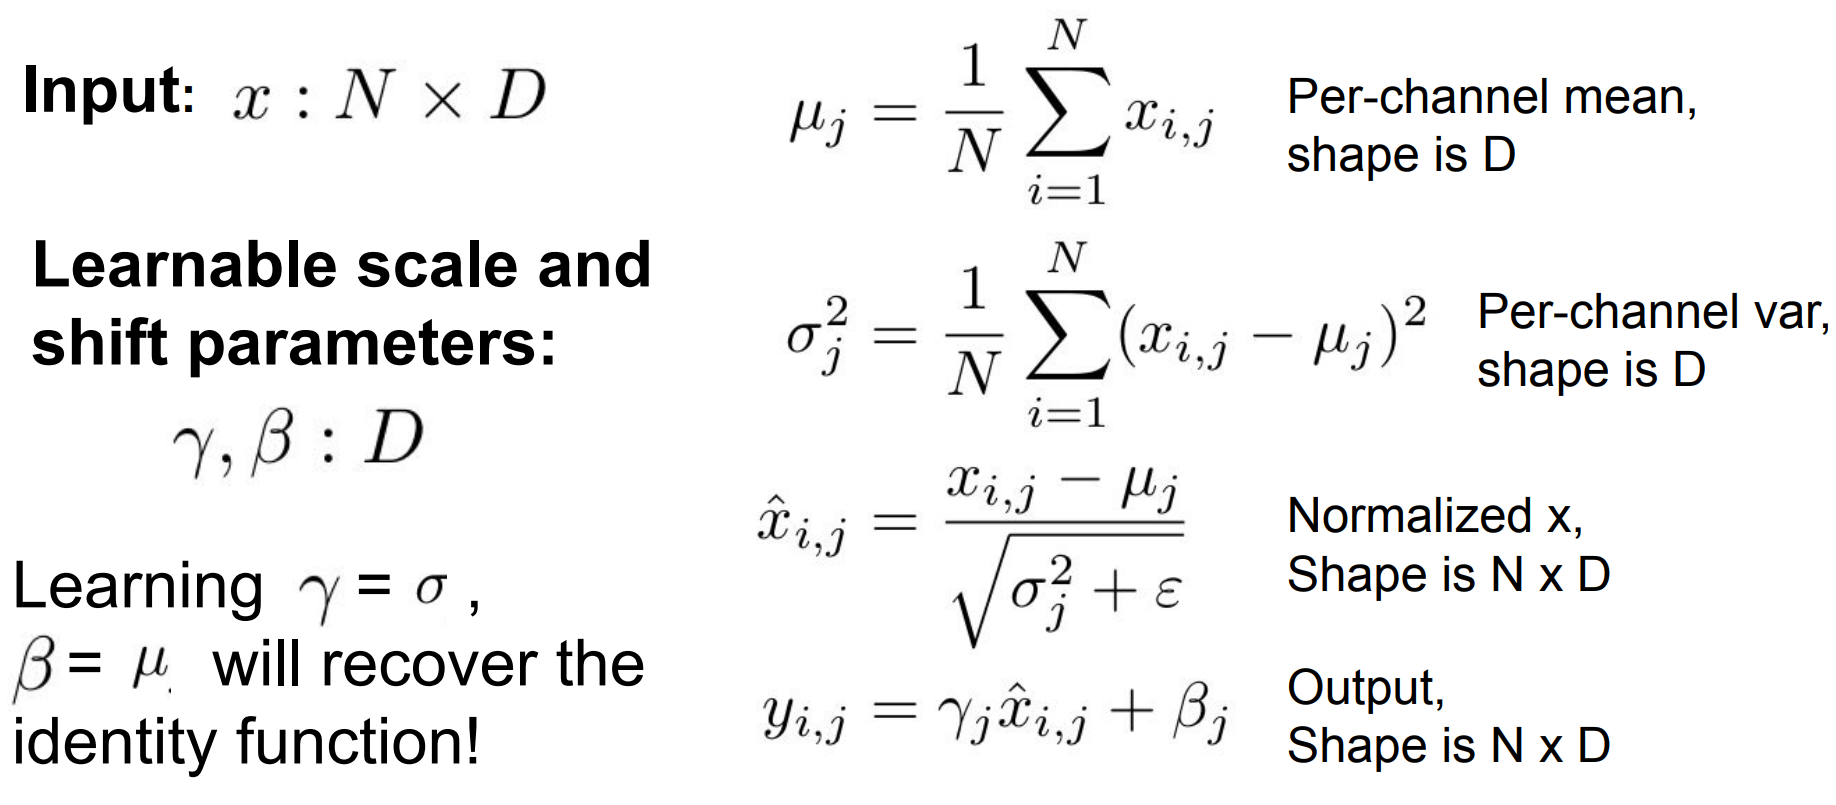
\includegraphics[width=1.0\textwidth,height=0.9\textheight,keepaspectratio]{images/cnn/batch_norm_1.png}
    \end{figure}
\framebreak
    \begin{figure}
    \centering
    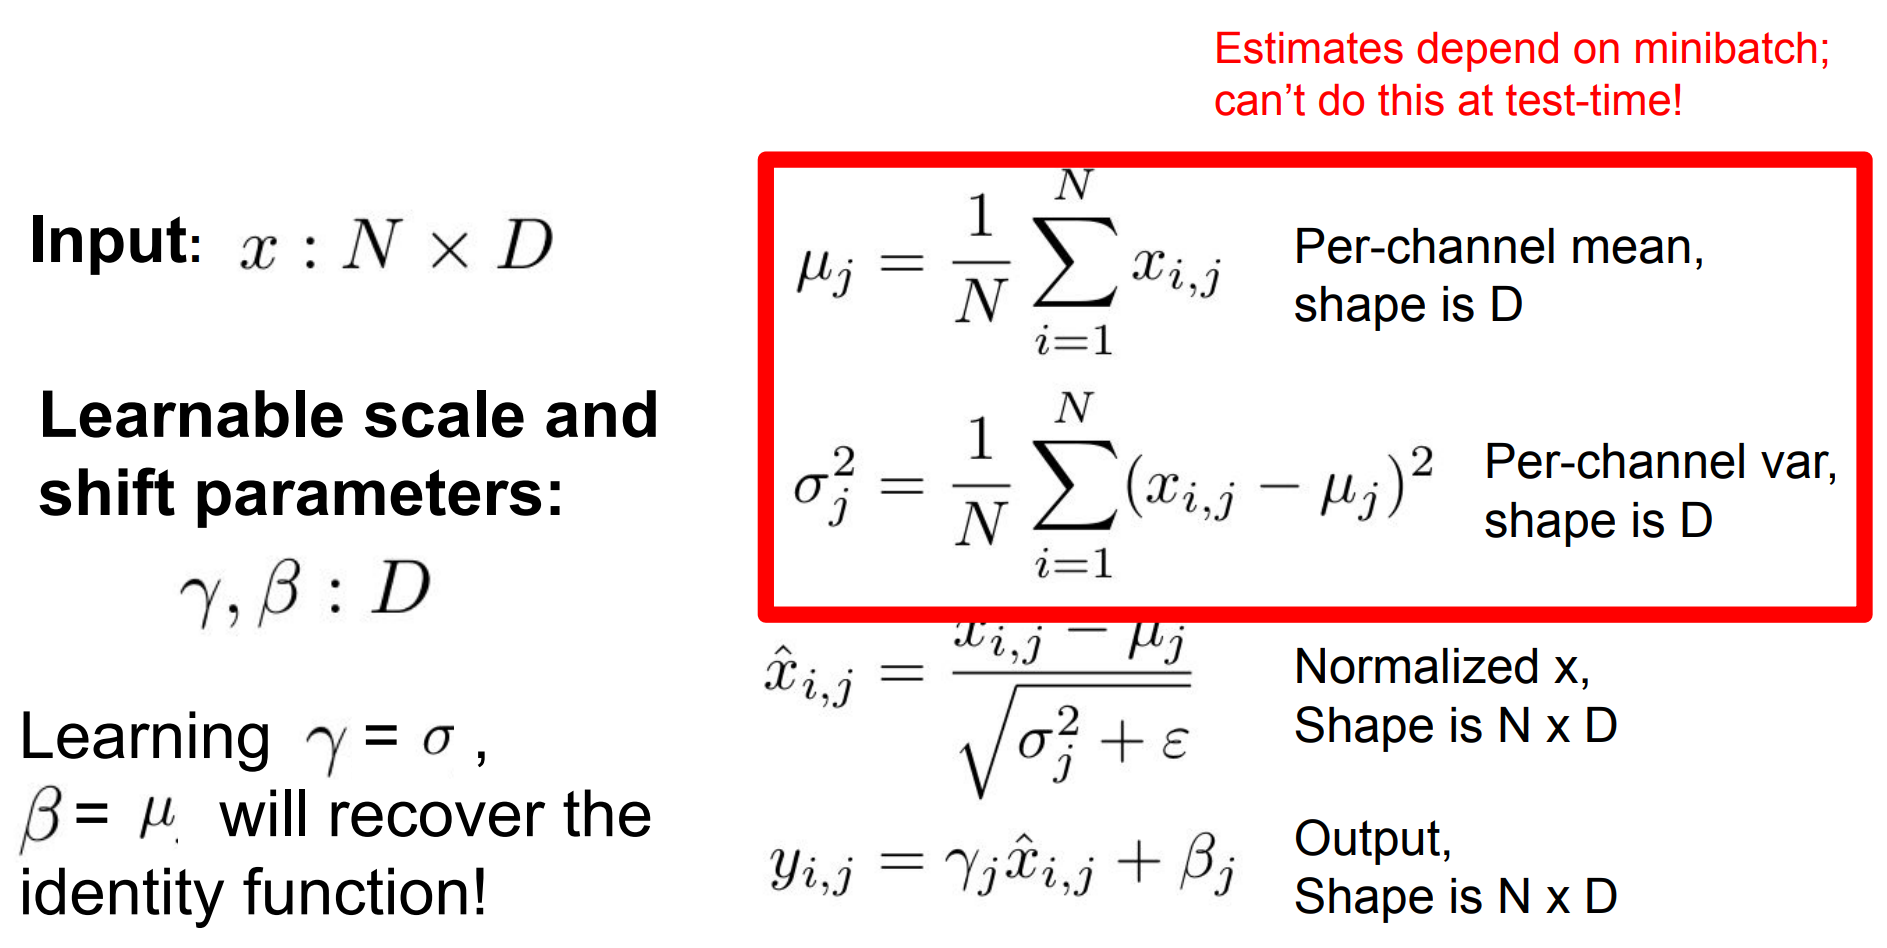
\includegraphics[width=1.0\textwidth,height=0.9\textheight,keepaspectratio]{images/cnn/batch_norm_2.png}
    \end{figure}
\framebreak
    \begin{figure}
    \centering
    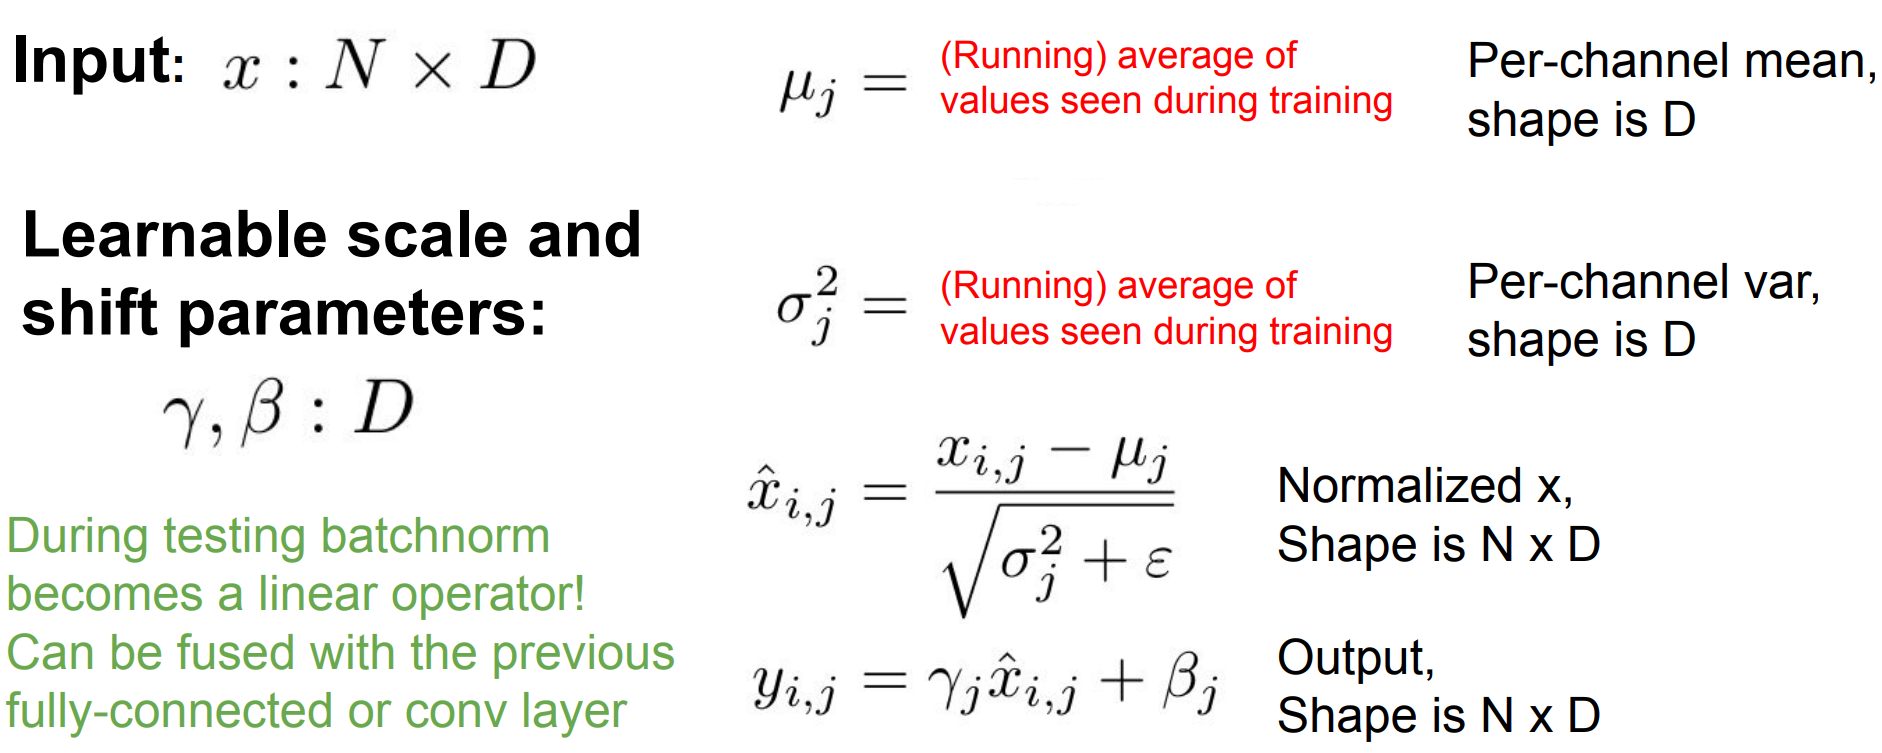
\includegraphics[width=1.0\textwidth,height=0.9\textheight,keepaspectratio]{images/cnn/batch_norm_3.png}
    \end{figure}
\framebreak
    \begin{figure}
    \centering
    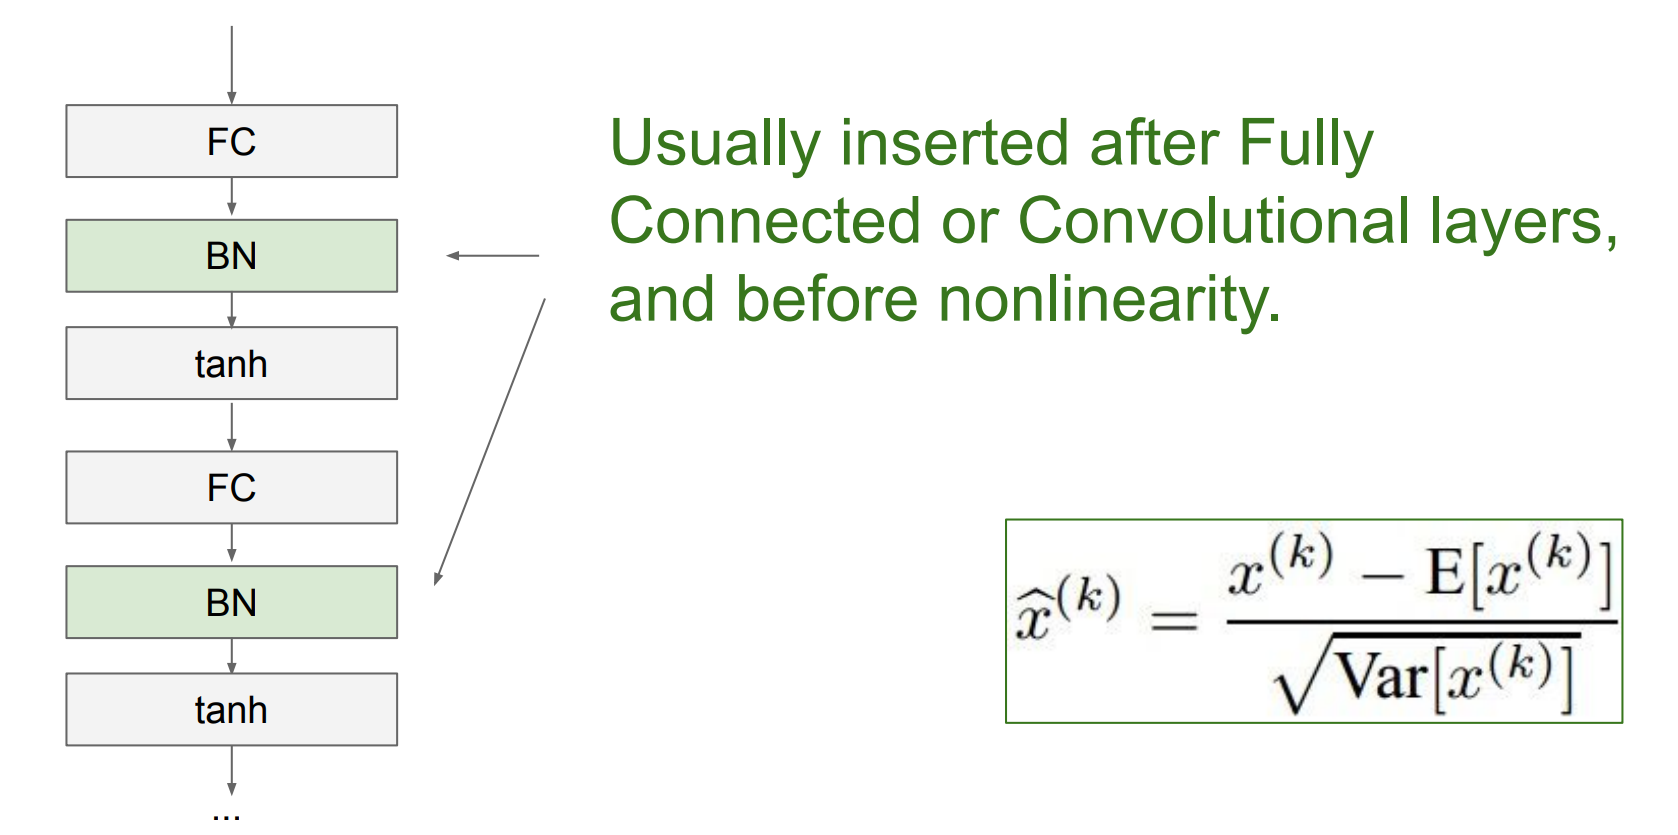
\includegraphics[width=1.0\textwidth,height=0.9\textheight,keepaspectratio]{images/cnn/batch_norm_4.png}
    \end{figure}
\framebreak
    \begin{figure}
    \centering
    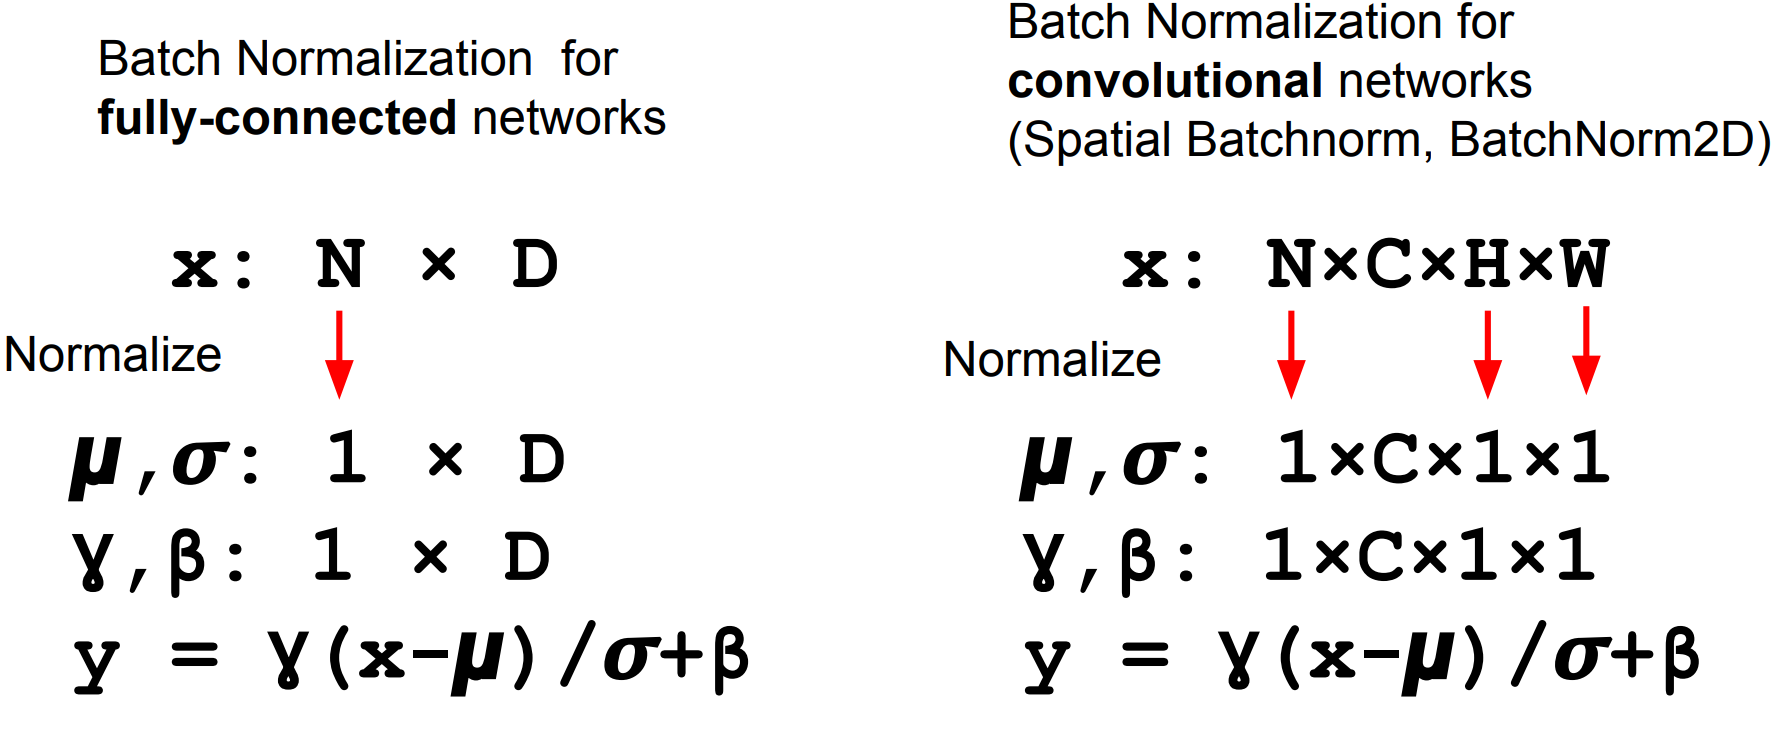
\includegraphics[width=1.0\textwidth,height=0.9\textheight,keepaspectratio]{images/cnn/batch_norm_5.png}
    \end{figure}
\framebreak
    \begin{itemize}
        \item Advantages:
        \begin{itemize}
            \item Makes deep networks much easier to train!
            \item Improves gradient flow
            \item Allows higher learning rates, faster convergence
            \item Networks become more robust to initialization
            \item Acts as regularization during training
            \item Zero overhead at test-time: can be fused with conv!
        \end{itemize}
        \pause
        \item Disadvantages:
        \begin{itemize}
            \item Behaves differently during training and testing: this is a very common source of bugs!
        \end{itemize}
    \end{itemize}
\end{frame}

\begin{frame}[fragile]{Normalization: Summary}
\begin{block}{What:}
    \begin{itemize}
        \item Normalize layer inputs over mini‑batch, then scale & shift.
    \end{itemize}
\end{block}

\begin{block}{Benefits:}
    \begin{itemize}
        \item Faster training,
        \item Allows higher learning rates,
        \item Reduces sensitivity to initialization,
        \item Acts as a regularizer.
    \end{itemize}
\end{block}

\begin{lstlisting}[language=Python, caption={Code snippet (PyTorch)}, basicstyle=\ttfamily\footnotesize]
import torch.nn as nn

bn = nn.BatchNorm2d(16)
x = bn(x)
\end{lstlisting}

\begin{block}{Note:}
    \begin{itemize}
        \item BatchNorm is typically used after convolutional layers and before activation functions.
        \item BatchNorm normalizes activations per‑batch, then scales/shifts them. 
    \end{itemize}
\end{block}
\end{frame}  

\begin{frame}{Normalization: Summary}
    \begin{figure}
    \centering
    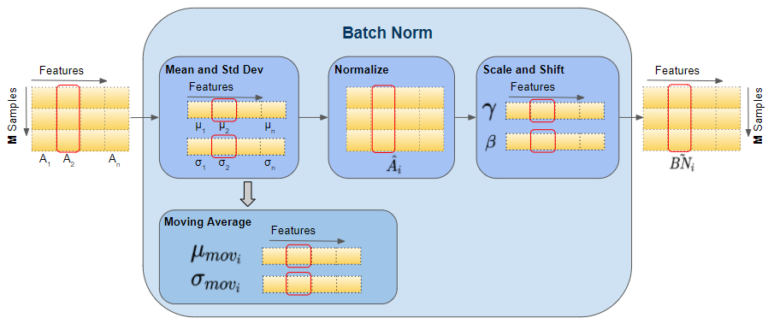
\includegraphics[width=0.95\textwidth,height=0.4\textheight,keepaspectratio]{images/cnn/batch-norm-unit.png}
    \end{figure}

    \begin{figure}
    \centering
    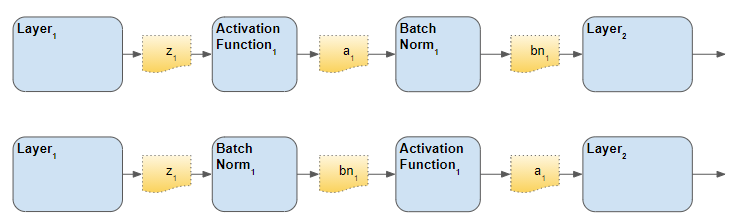
\includegraphics[width=0.95\textwidth,height=0.4\textheight,keepaspectratio]{images/cnn/batch-norm-sequence.png}
    \caption*{Order of placement of Batch Norm layer}
    \end{figure}
    \vspace{-0.5cm}
    \href{https://towardsdatascience.com/batch-norm-explained-visually-how-it-works-and-why-neural-networks-need-it-b18919692739/}{More on Batch Norm from Towards Data Science}
\end{frame}